In July 2000, the NIH Biomedical Information Science and Technology Initiative Consortium released a document \cite{huerta_nih_2000} 
through which they defined bioinformatics as “Research, development, or application of computational tools and approaches 
for expanding the use of biological, medical, behavioral or health data, including those to acquire, store, organize, 
archive, analyze, or visualize such data.”

Bioinformatics is a highly interdisciplinary field. Figure~\ref{fig:bioinformaticsDisciplines} shows the Interaction 
of various disciplines that have contributed to the formation of bioinformatics \cite{bayat_science_2002}. 
It conceptualizes biology in terms of macromolecules and aims to extract knowledge from the information associated with 
these molecules on a large-scale. It extracts the intended information by applying "informatics" techniques 
(derived from various disciplines such as statistics, computer science, maths, linguistics, etc.) to the biological data. 
Depending on the goal of the study, the biological data could be collected from sources such as information stored in the 
genetic code, experimental results, patient statistics, scientific literature, etc. 
\cite{nilges_bioinformatics-definition_2011,luscombe_what_2001}.

\begin{figure}[ht]
    \centering
    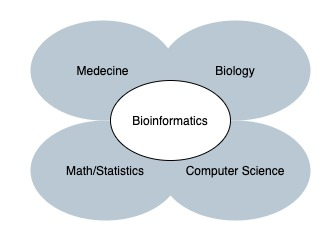
\includegraphics[width=0.60\textwidth]{figures/05Bioinformatics.jpg}
    \caption{Disciplines contributed to the formation of bioinformatics reproduced from~\cite{bayat_science_2002}}
    \label{fig:bioinformaticsDisciplines}
\end{figure}


With the exponential growth in the amount of available biological data, research in bioinformatics should be able to 
address method development for both data management (e.g. storage, retrieval of data) and extraction of useful information 
from these data (data analysis). One of the main challenges in bioinformatics is development of the tools and methods capable 
of transforming data into biological knowledge which is the focus of the second area being mentioned above. These tools and 
methods should be able to extract knowledge in the form of testable models. By this simplifying abstraction that constitutes 
a model, we will be able to predict the behavior of the system. In modern biology and medicine, bioinformatics is essential 
and has many practical applications in different areas of those fields.

One of the popular data analysis tools by which researchers try to predict the behavior of a system is “Machine Learning”. 
It is a direct descendant of statistical model fitting. 
Machine learning tries to extract useful information from a set of data by building good probabilistic models. However,  
according to~\cite{baldi_bioinformatics_2001},
\begin{quote}
the particular twist behind machine learning, is to automate this process as much as possible, often by using 
very flexible models characterized by large numbers of parameters, and to let the machine take care of the rest
\end{quote}
In a problem, the term “learning” refers to running a computer program to induce a model by using training data or 
past experience.  Machine-learning approaches are best suited for areas where there is a large amount of data 
but little theory which is exactly the situation in computational molecular biology \cite{chauvin_backpropagation_1995}.

\begin{figure}[ht]
    \centering
    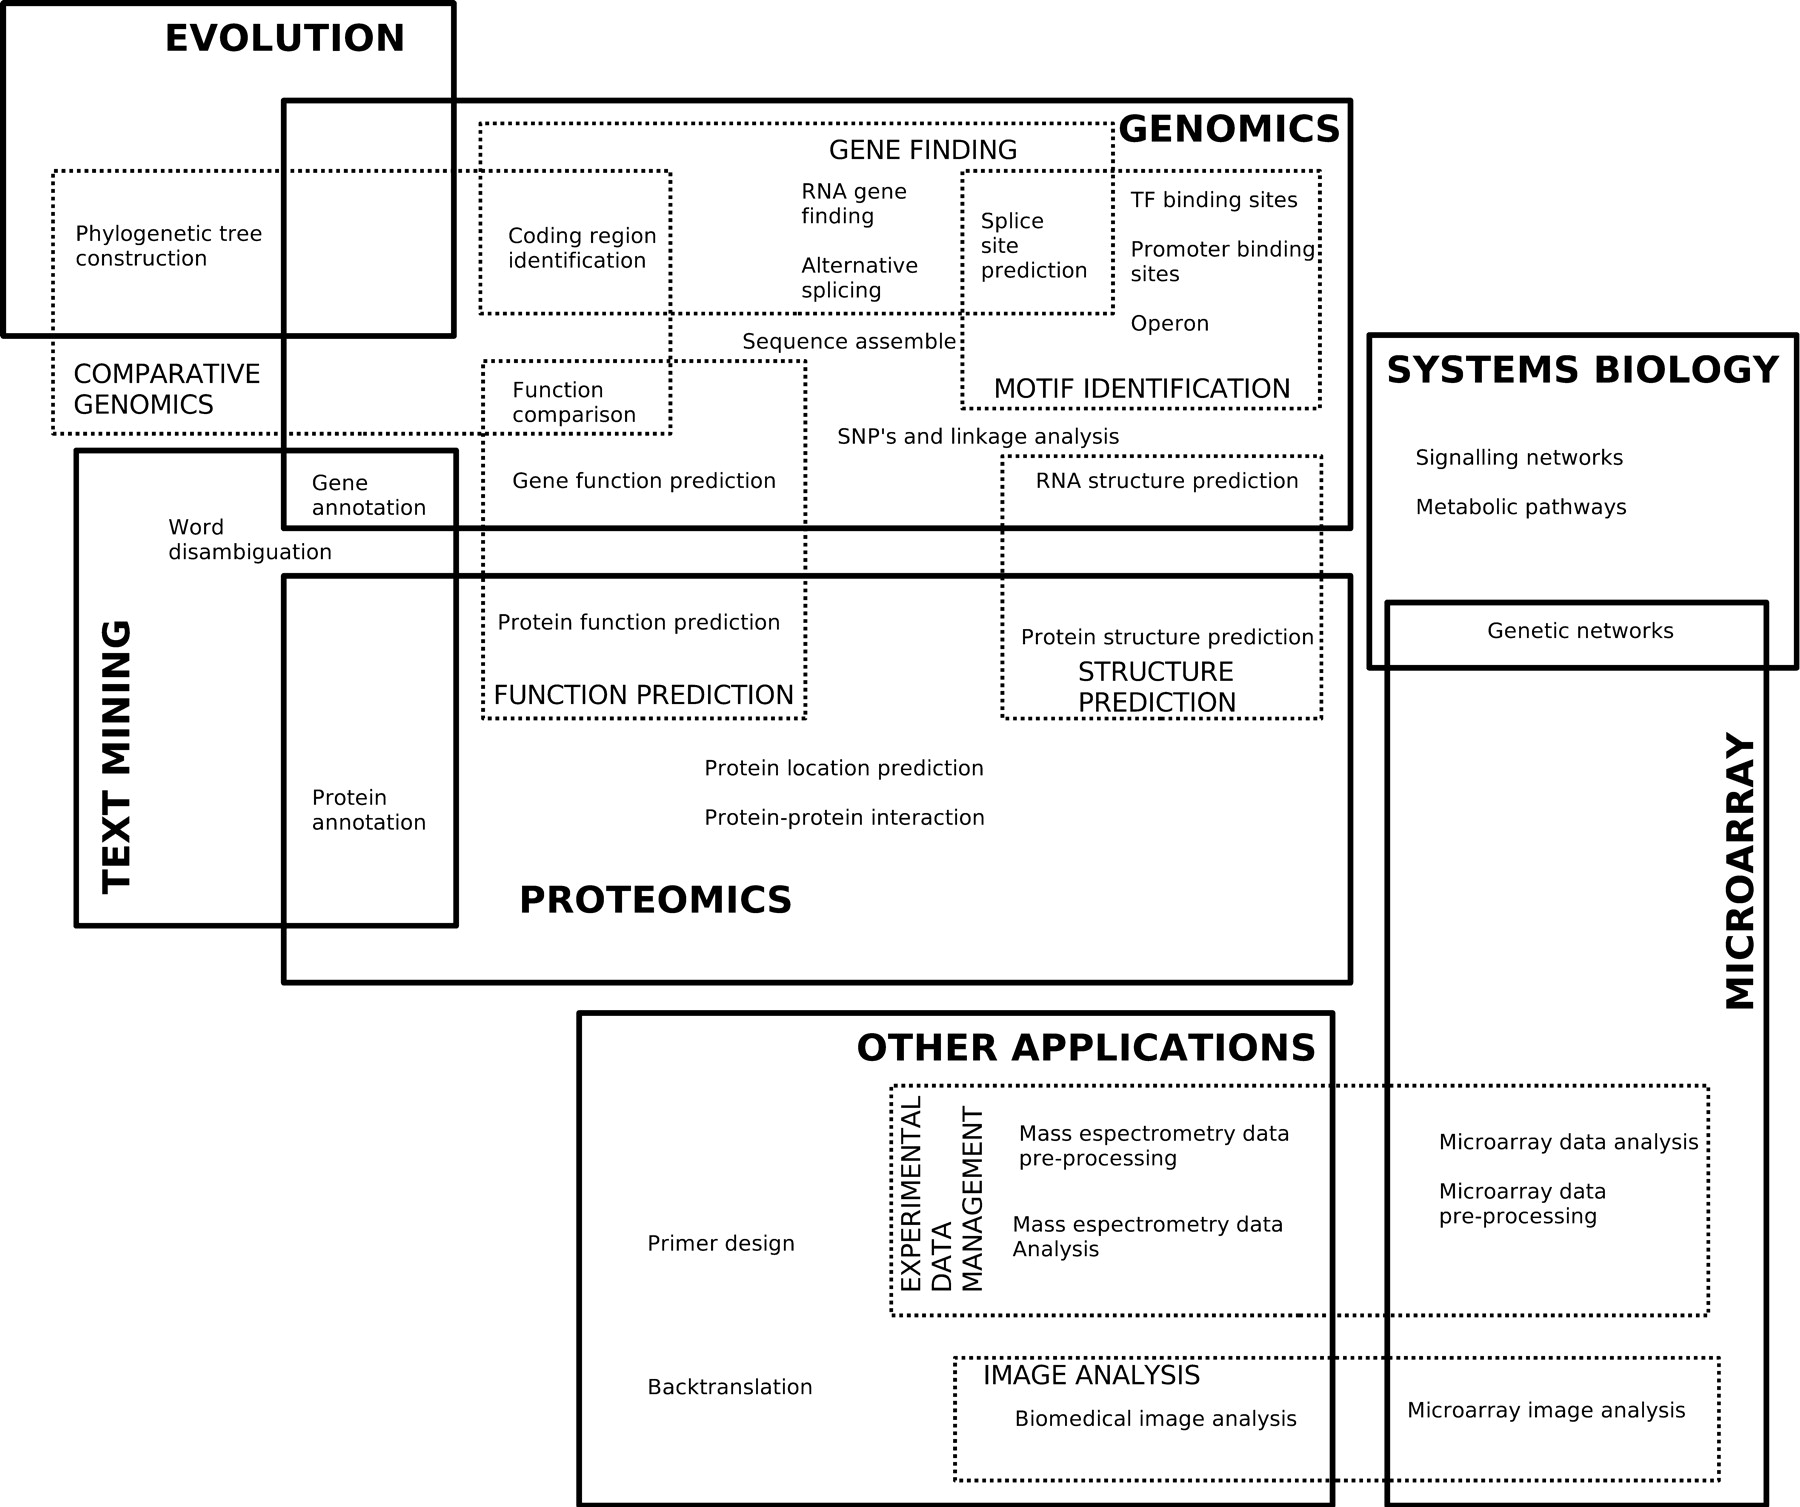
\includegraphics[width=0.70\textwidth]{figures/06BioinformaticsTopics.jpg}
    \caption{Main biological problems where computational methods are applied 
    extracted from~\cite{larranaga_machine_2006}}
    \label{fig:bioinformaticsTopics}
\end{figure}

There are various biological domains where computational methods and techniques are applied for data analysis and knowledge 
extraction from the data. Pedro Larrañaga et al. \cite{larranaga_machine_2006} have classified those problems into 
following domains: genomics, proteomics, microarrays, systems biology, evolution and text mining. 
Figure~\ref{fig:bioinformaticsTopics} shows the main biological problems where machine learning and computational methods 
are being applied. The “other applications” category includes all the remaining problems besides the ones mentioned above.

In the proteomics domain, supervised machine learning techniques are used for protein structure prediction and protein 
function prediction \cite{lesh_complete_2003,mishra_prediction_2014}. As a subcategory of machine learning, supervised 
learning is defined by its use of labeled datasets for training the algorithm that is supposed to classify data or 
predict the outcome accurately. Unlike supervised learning, unsupervised learning tries to discover patterns in an unlabeled 
set of data.

Since extraction and annotation of the protein sequences are a time consuming and expensive process, the researchers 
often have to build and train models on imbalanced datasets (imbalanced learning). As we mentioned earlier, bioinformatics 
is a highly interdisciplinary field. With the new achievements in the related fields (e.g. sequencing, machine learning), 
researchers should be able to apply new techniques to the fairly older problems to see if those new techniques could improve 
results or solve the problem. In the case of machine learning, new achievements can provide the researchers with more data 
which can improve learning and eventually the model performance.

Due to the reasons mentioned above, along with the fact that bioinformatics research in some areas directly deals 
with humans health (e.g. medicine), like some other fields of studies with similar characteristics (e.g. psychology), 
reproducible research has received a notable amount of attention through the past decade 
\cite{tatman_practical_2018,mcdermott_reproducibility_2019}. Reproducibility plays an important role as a 
tool for both claim verification and research improvement and adjustment. 

In the case of imbalanced learning (which is the focus of this study), a researcher needs to take some extra steps 
(compared to machine learning problems on a balanced set of data) for building the model and predicting the final outcome. 
Since there are more parameters involved, we believe in similar problems, the study report should also include details on 
these important parameters to ensure high degree of reproducibility. Otherwise, older studies need to be remodeled and 
programmed from scratch which could be time consuming, expensive and sometimes may not be possible since some resources 
being used in the initial study may not be available anymore.

The following section will provide a brief introduction to the supervised classification of imbalance data 
(imbalanced learning). We will briefly review the corresponding concepts, how imbalanced data classes could affect the 
learning process, performance metrics and suggested solutions for similar problems through different domains of studies. 
The section intends to picture how balanced classification is different from the imbalanced one which is the focus of this study.
